%!TEX root = ../../Main.tex
\graphicspath{{Chapters/Struktur/}}
%-------------------------------------------------------------------------------

\section{Struktur}

I dette projekt er der taget et valg udfra læringsmålene om at vi bruger Blackfin platformen til at udføre projektetes funktionalitet. Da en blackfin processor er bygget op af mange funktionalle blokke, vil der i det kommende afsnit laves et overblik over de hardware blokke som bliver brugt i dette projekt. 

\begin{figure}[H]
	\centering
	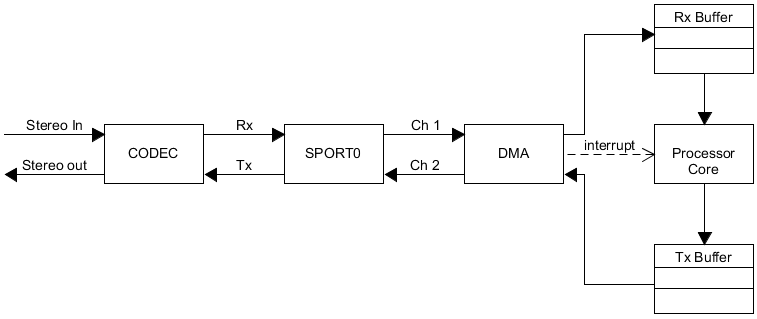
\includegraphics[width = 400pt]{Img/Struktur}
	\caption{Struktur NSS}
	\label{fig:LMS_filter}
\end{figure}

Igennem processen af vores funktionalitet, sendes lydsignalet gennem en codec1836, som har til opgave at sende inputtet gennem en ADC, hvorefter den sender det digitale signal videre til SPORT0, som står for at forbinde de interne blokke, igennem dette projekt bruger vi den interne clock, hvor frekvensen kan beregnes ud fra formlen:

\begin{figure}[H]
	\centering
	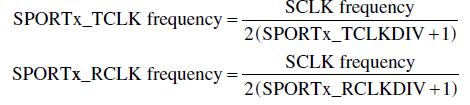
\includegraphics[width = 300pt]{Img/Frekvens}
	\caption{Formel for clock frekvens}
	\label{fig:LMS_filter}
\end{figure}
  
Systemet fører herefter signalet til DMA'en som står for at placerer dataen i de rigtige registre i memory. Herefter sker selve proceceringen af dataen, hvor vores funktionalitet er implementeret. Det filtrede og bearbejde signal sendes herefter den modsatte vej og kommer igennem alle blokke igen og ender som et analogt signal på udgangen. 

\newpage

